%%%%% START PREAMBLE HEADER %%%%%

%%% START REQUIRED PACKAGES %%%

\documentclass[twocolumn]{article}
\usepackage{xcolor} 
\usepackage[a4paper, total={7.25in, 9.5in}]{geometry} 
\usepackage{multirow}
\usepackage{lipsum}
\usepackage{hyperref}
\usepackage{listings}
\usepackage{graphicx}
\usepackage[export]{adjustbox}
%\usepackage[superscript,biblabel]{cite}
\usepackage{amsmath}
\hypersetup{colorlinks=true,linkcolor=blue,filecolor=magenta,urlcolor=cyan,citecolor=blue}

%%% END REQUIRED PACKAGES %%%                


%%% START NEW COMMANDS new (shortcut) %%%

% This is a paragraph with normal font
\newcommand{\np}[1]{\paragraph*{\normalfont{#1}}}
% This is a text with a color
\newcommand{\ct}[2]{\textcolor{#1}{#2}}
% This is a bold text 
\newcommand{\bt}[1]{\textbf{#1}}
% This is an italic text 
\newcommand{\et}[1]{\emph{#1}}
% This is an underline text 
\newcommand{\ut}[1]{\underline{#1}}
% This is a newline shortcut
\newcommand{\n}{\\}
% This is a numbered equation with break line shortcut
\newcommand{\necbreak}[1]{\begin{equation}\begin{aligned}#1\end{aligned}\end{equation}}
% This is a numbered equation with break line shortcut
\newcommand{\nec}[1]{\begin{equation}#1\end{equation}}
% This is an equation shortcut
\newcommand{\ec}[1]{\begin{center} $#1$ \end{center}}
% Table title with bold text and correct space%
\newcommand{\titleTable}[2]{\np{\bt{Table #1} #2}}% Graph title with bold text and correct space%
\newcommand{\titleGraph}[2]{\np{\bt{Graph #1} #2}}
% Table body with border %
\newcommand{\bodyTable}[2]{\begin{center} \begin{tabular}{|#1|} \hline #2 \hline \end{tabular} \end{center} }
%%% END NEW COMMANDS (shortcuts) %%%


%%% START TITLE SETTINGS %%%
\title{State transition and rate constant}
\author{Perez Alvarado Luis Raymundo, School of Chemistry, UNAM}
\date{08/10/2020}
%%% END TITLE SETTINGS %%%

%%%%% END PREAMBLE HEADER %%%%%

%%%%%%%%%%%%%%%% START DOCUMENT %%%%%%%%%%%%%%%%
\begin{document}

    %%% THIS CONTENT IS IN ONE COLUMN (START) %%%
    \twocolumn[
        \begin{@twocolumnfalse}

            %% CREATE A TITLE (START) %%
            \maketitle
            %% CREATE A TITLE (END) %%

            %% CREATE A ABSTRACT (START,MAX 250 CHARACTERS) %%
            \begin{abstract}
                \item 
                \item 
            \end{abstract}
            %% CREATE A ABSTRACT (END) %%
    
        \end{@twocolumnfalse}
    ]
    %%% THIS CONTENT IS IN ONE COLUMN (END) %%%

    %%% THIS CONTENT IS IN TWO COLUMN (START) %%%

    %% START SECTION %%

    % SECTION TITLE %
    \section*{Introduction}

    \np{Hartree-Fock(HF) is one of the most famous methods of approximation to the determination of the wave function and energy for a quantum many-body system.\cite{web:wiki} }

    \np{HF approximation is used to solve the Schrödinger equation, this is the general form.}

    \nec{\hat{H}\Psi=E\Psi \label{eq:equation 1}}

    \np{The Hamiltonian operator in Schrödinger equation independent of time.}
    
    \necbreak{\label{eq:equation 2}
        \hat{H}= & \frac{n^2}{2}\sum_{\alpha}\frac{1}{m\alpha}\nabla^2_{\alpha}-\frac{n^2}{2m}\sum_{i}\nabla^2_{i}+\sum_{\alpha}\sum_{\alpha>\beta}\frac{z_{\alpha}z_{\beta}e^2}{r_{\alpha\beta}}\\
        & \sum_{\alpha}\sum_{i}\frac{z_{\alpha}e^2}{r_{\alpha i}}+\sum_{i}\sum_{i>j}\frac{e^2}{r_{ij}} 
    }

    \np{Where the last term of the equation \eqref{eq:equation 2} represents the repulsion of electrons and does not have an exact solution, in the approximation made in HF it is proposed that each electron be considered an average density of all the others electrons.\cite{web:hf}\cite{web:Washington}}
    
    
    \np{The difference between the exact nonrelativistic energy ($E_{nonrel}$) and the energy using HF($E_{HF}$) is called correlation energy($E_{corr}$), this term is a consecuence of the repulsion of $n$ electrons.\cite{inbook:QuantumChem}}
    
    \nec{E_{corr}=E_{nonrel}-E_{HF}\label{eq:equation 3}}

    \np{The enthalpy of formation ($\Delta H_{f}$) calculation is an example of the things that can be done using computational chemistry, solving equation \eqref{eq:equation 1} the thermodynamic properties can be calculated and use in Hess's law to obtain $\Delta H_{f}$.\cite{web:hess}}
    
    \nec{\Delta H_{formation}=\Delta H_{f products}-\Delta H_{freactives}\label{eq:equation 4}}

    \section*{Methods}

    \np{The modeling of the systems $CH_{4}$,$\cdot OH$,$TS$,$CH_{3}\cdot$ and $H_{2}O$ was performed with gaussView separately.}

    \np{In the input file with extension .gjf /.com, the following settings was used for $F$ and $F_{2} $ to perform a calculation with the HF method. \n}

    % START FIGURE %
    \begin{figure}[h]
        % Reactive %
        \centering
        \begin{minipage}[b]{0.225\textwidth}
            \centering
          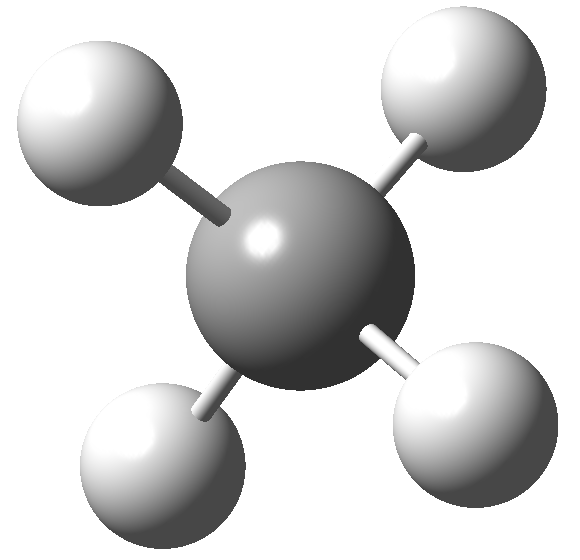
\includegraphics[scale=0.55]{methane.png}
          \caption{Methane.}
        \end{minipage}
        \hfill
        \begin{minipage}[b]{0.25\textwidth}
          \centering
          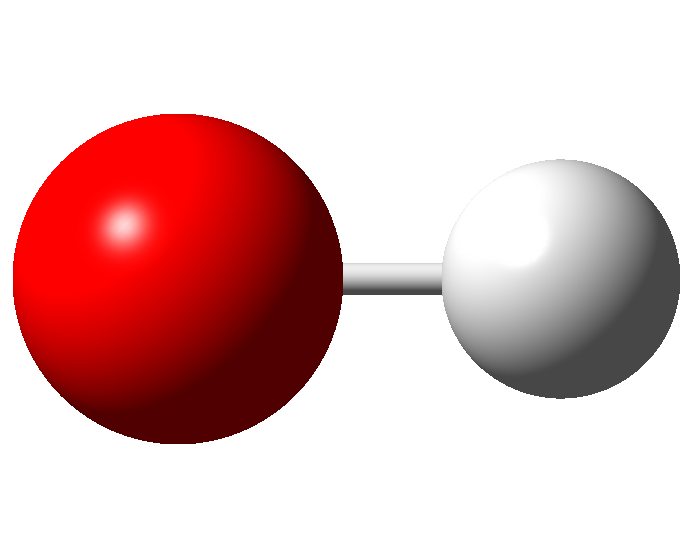
\includegraphics[scale=0.4]{hidroxilRadical.png}
          \caption{Hydroxyl radical.}
        \end{minipage}
        %Transition state%
        \begin{minipage}[b]{0.45\textwidth}
            \centering
            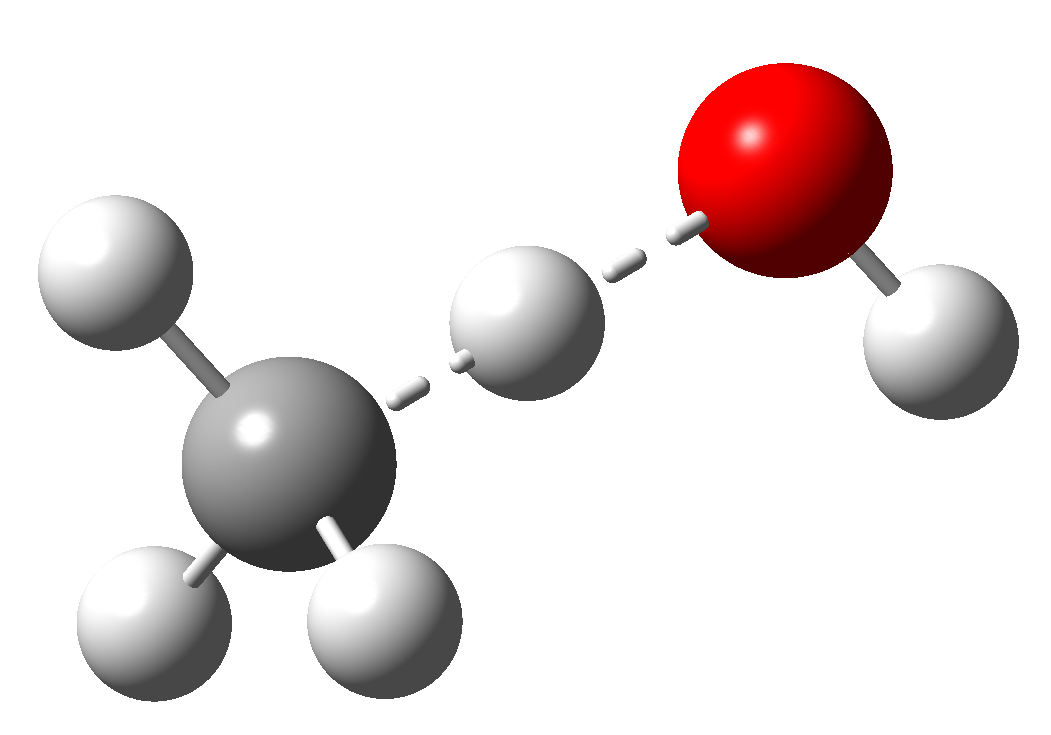
\includegraphics[scale=0.575]{stateTransition.png}
            \caption{Transition state.}
        \end{minipage}
        %products%
        \centering
        \begin{minipage}[b]{0.225\textwidth}
            \centering
          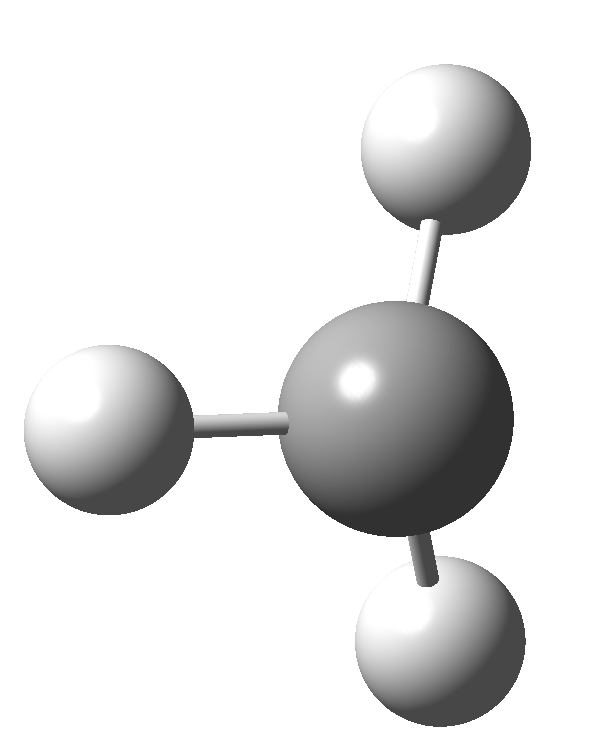
\includegraphics[scale=0.55]{methylRadical.png}
          \caption{Methyl radical.}
        \end{minipage}
        \hfill
        \begin{minipage}[b]{0.25\textwidth}
          \centering
          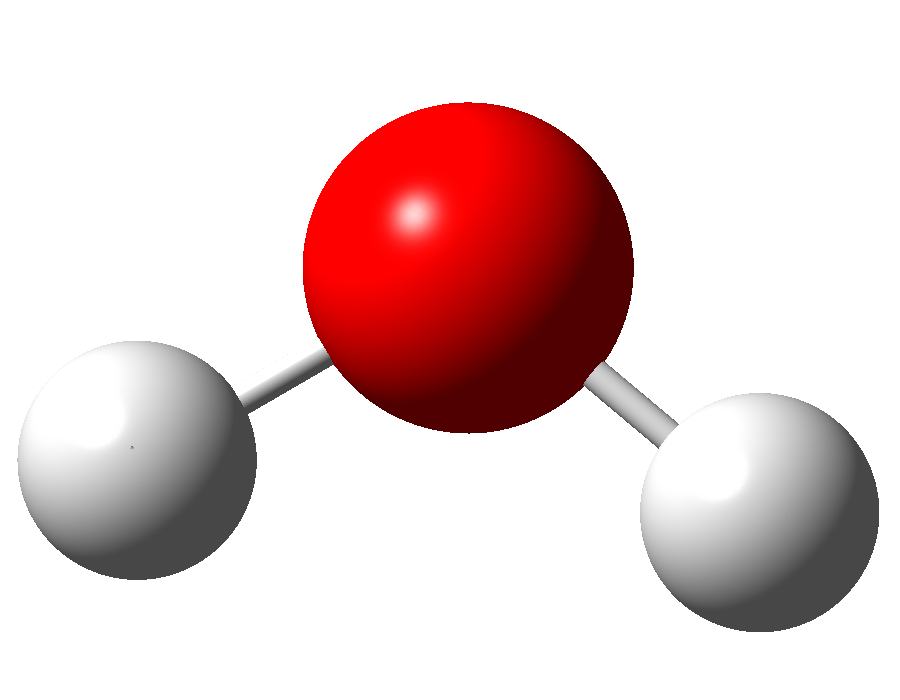
\includegraphics[scale=0.4]{water.png}
          \caption{Water.}
        \end{minipage}
    \end{figure}
    % END FIGURE %
    \nec{ CH_{4}+\cdot~ OH \rightarrow [ CH_{3}\mbox{-}~\mbox{-}H\mbox{-}~\mbox{-}OH]^{\dagger} \rightarrow CH_{3}\cdot+H_{2}O}

    \np{The global reaction is describe in 5\n}
    


    \begin{lstlisting}[frame=single,gobble=10] 
            //hardware configuration
            % nprocshared=4
            % mem=1500MB
            //parameters for Hartree-Fock method
            # opt freq HF/6-31+g(d) 
    \end{lstlisting}

    \np{The calculations of the $F$ and $F_{2}$ systems were performed with HF.}
    
    \np{After finish calculations with HF, the procedure was repeated with B3LYP and MP2 methods, and use the same hardware configuration and the same base set and just change the method.\n}

    \begin{lstlisting}[frame=single,gobble=10] 
            //parameters for B3LYP method
            # opt freq B3LYP/6-31+g(d)
            //parameters for MP2 method
            # opt freq MP2/6-31+g(d)
    \end{lstlisting}    
    
    \np{\bt{NOTE:} In the case of F is not necessary to use opt configuration because does not need geometry optimization.}
    
    \section*{Results}
    
    \np{Through the data calculated in table 2, the reaction profile was plotted (Fig 2)}

    \titleGraph{1}{Free energy VS Reaction coordenate}

    \np{Through the data calculated in table 2, the reaction profile was plotted (Fig 1)}

    \vspace{-0.5cm}
    \begin{figure}[h]
        \centering
        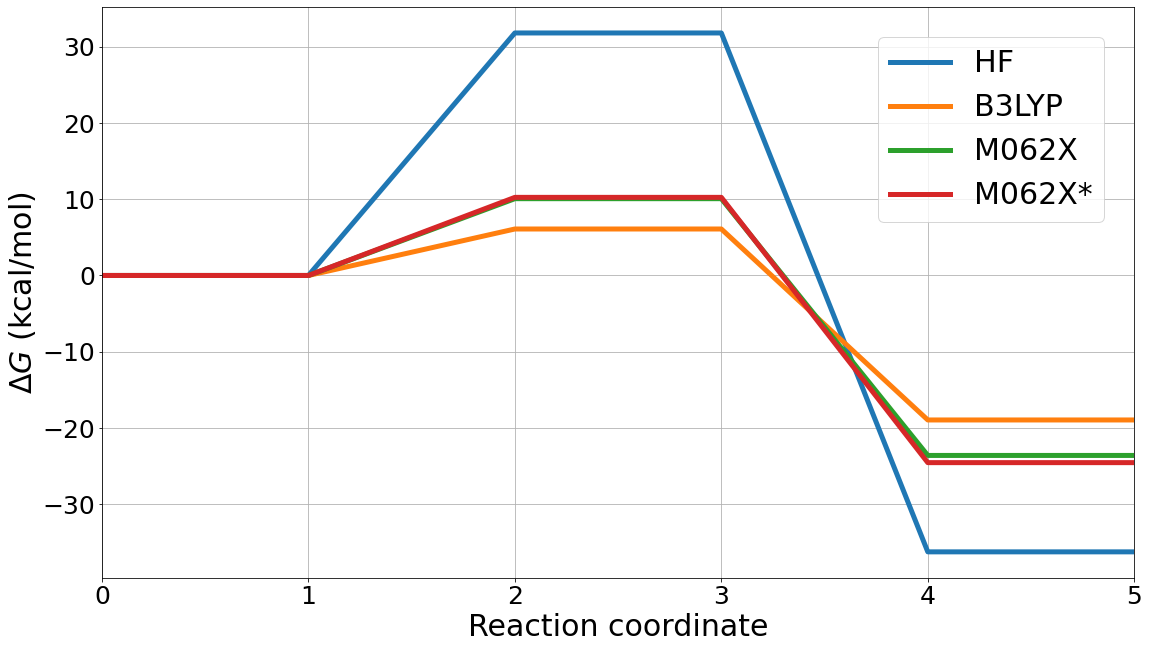
\includegraphics[width=0.49\textwidth]{reactionProfileFreeEnergy.png}
        \caption{Profile reaction.}
    \end{figure}

    \titleGraph{2}{Enthalpy VS Reaction coordenate}

    \np{asdasd}

    \vspace{-0.5cm}
    \begin{figure}[h]
        \centering
        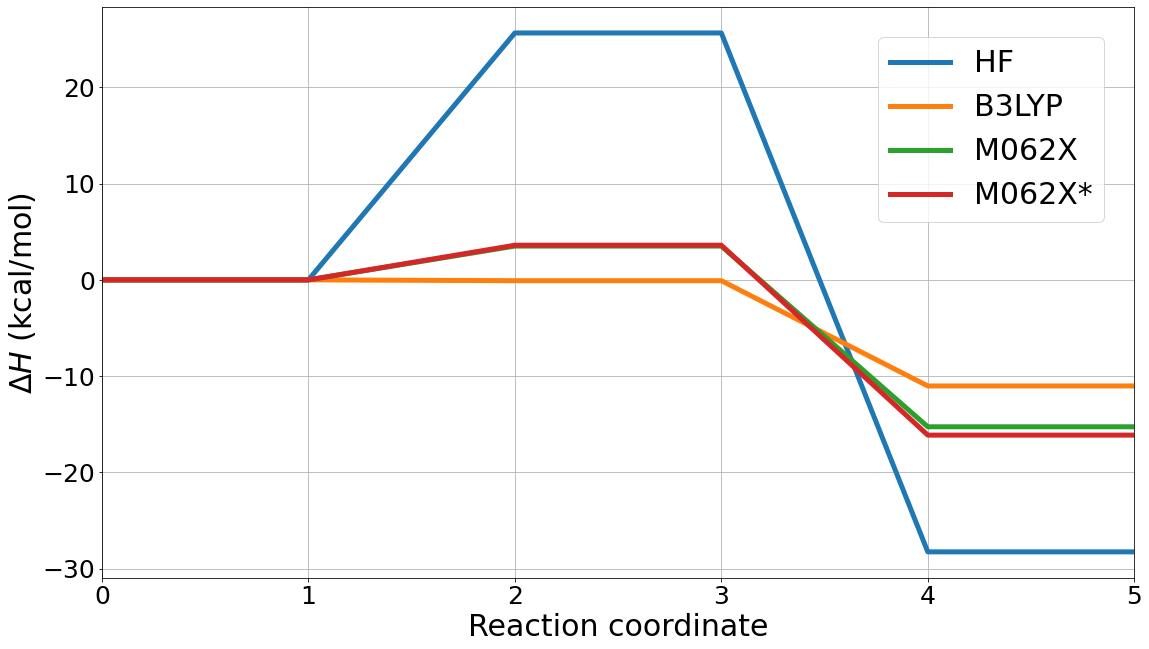
\includegraphics[width=0.49\textwidth]{reactionProfileEnthalpy.png}
        \caption{Profile reaction.}
    \end{figure}




    % START A TABLE %
    % TABLE TITLE %
    \titleTable{1}{ETE values for HF, B3LYP, and MP2 methods using the 6-31G basis set and time($t$) of each calculation.}

    % TABLE BODY %
    \bodyTable{c|c|c|c|c}{
        \bt{Method} & \bt{$\Delta H_{F}(H_{E})$} & $t_{F}(s)$ & \bt{$\Delta H_{F_{2}}(H_{E})$} & $t_{F_{2}}(s)$ \n
        \hline
        HF & -99.369 & 2.000 &-198.678 & 6.000 \n 
        \hline
        MP2 & -99.496 & 10.000 & -199.047 & 19.000 \n 
        \hline
        B3LYP & -99.7282 & \ct{blue}{2.000} & -199.511 & \ct{blue}{6.000}\n        
    }
    % END A TABLE %

    \np{Using equation \eqref{eq:equation 4} the enthalpy of formation of the $F_{2}$ is calculated.}

    \ec{\Delta H_{f_{(F_{2})}}=\Delta H_{F_{2}}-2\Delta H_{F}}

    \np{Using the factor of conversion $627.509\frac{kcal}{mol}$ \cite{web:factorConv} $H_{E}$ units of $\Delta H_{f}$ are converted into $\frac{kcal}{mol}$.}

    \np{Knowing a reference value that is  $-158.739\frac{kJ}{mol}$ \cite{web:refValue} the error percentage is calculated for each method.}

    % START A TABLE %
    % TABLE TITLE %
    \titleTable{2}{Enthalpy of formation of $F_{2}$ calculated with HF, MP2, and B3LYP methods and his percentage error.}

    % TABLE BODY %
    \bodyTable{c|c|c|c}{
        \bt{Method} & \bt{$\Delta H_{f_{(F_{2})}}(H_{E})$} & \bt{$\Delta H_{f_{(F_{2}})}(\frac{kcal}{mol})$} & \bt{\%Error}\n 
        \hline
        HF & 0.060 & 37.705 & \bt{47.653} \n 
        \hline
        MP2 & -0.054 & -34.262 & 2.316 \n 
        \hline
        B3LYP & -0.055 & -34.577 & \ct{blue}{2.117}\n        
    }
    % END A TABLE %
    \np{\bt{NOTE:} The reference value was used in $\frac{kcal}{mol}$ in the determination of $\%Error=\frac{| valCalc-valRef |}{valRef}\cdot 100 \% $, and all decimals were used during the calculations, but was rounded to 3 significant decimal places.}

    \section*{Discussion}

    \np{Comparing the percentage of error of each method can see those post-HF methods, in this case, B3LYP is based in \et{density Functional Theory}(DFT) and MP2 based in \et{Perturbation Theory} have an acceptable error, but the error of the HF method is not acceptable at all!, this is because HF does not consider the $E_{corr}$, and this is the reason why \bt{HF it is useless} for the calculation of systems with more than one electron.}

    \np{In this particular case to calculate the thermodynamic properties of $ F_ {2} $ and $ F $ the best method using the set of bases 6-31G is \bt{B3LYP} considering that the percentage error is the lowest compared to the others two and has a low computational cost.}

    %% END SECTION %%
    

    %% START REFERENCES %% 

    % DEFINE STYLE FORMAT%
    \bibliographystyle{ieeetr}
    % SPECIFY THE FILE NAMEw %
    \bibliography{references}

    %% END REFERENCES %% 

    %%% THIS CONTENT IS IN TWO COLUMN (END) %%%

\end{document}
%%%%%%%%%%%%%%%% END DOCUMENT %%%%%%%%%%%%%%%%